\documentclass[12pt,a4paper]{article}
\usepackage{amsmath}
\usepackage{mathtext}
\usepackage{icomma}
\usepackage{amsfonts}
\usepackage{amssymb}
\usepackage[utf8]{inputenc}
\usepackage[T1,T2A]{fontenc}
\usepackage[english, russian]{babel}
\usepackage{graphicx}
\usepackage[left=2cm,right=2cm,top=2cm,bottom=2cm]{geometry}
\usepackage{calc}
\usepackage{wrapfig}
\usepackage{setspace}
\usepackage{indentfirst}
\usepackage{subfigure}
\usepackage[table,xcdraw]{xcolor}
\usepackage{float}

\title{Отчет о проектной деятельности. \\
Моделирование магнитного поля в окрестности образцов.}

\author{Исламов Сардор, группа Б02-111}
\date{}

\begin{document}
\maketitle
\subparagraph*{Аннотация.} В работе на основе закона Био-Савара-Лапласа и методов численного интегрирования в среде MATLAB промоделированы магнитные поля от произвольных типов образцов, описываемых множеством точек в пространстве.  
Также просчитана траектория заряженных частиц в таких полях. 

\subsection*{Теоретическое введение}
\subparagraph*{Закон Био-Савара-Лапласа.} Сформулируем закон, определяющий магнитное поле движущегося точечного заряда $q$, ограничиваясь при этом равномерными движениями с малыми скоростями ($v \ll c$).
Закон получается обобщением опытных фактов и выражается формулой 
\begin{equation}
    \textbf{B} = {q \over c r^3} [\textbf{v} \times \textbf{r}],
\end{equation}

где \textbf{r} -- радиус-вектор, проведенный от заряда $q$ к точке наблюдения, $c$ -- электродинамическая постоянная, которая, в ходе исследований, оказалась равной скорости света в вакууме. 
При переходе в гауссову систему измерений СГС коэффициент пропорциональности $c$ пропадает.

Электрическое поле неподвижного (или медленно движущегося) заряда той же величины $q$ в той же точке наблюдения определяется выражением 
\[ \textbf{E} = {q \over r^3} \textbf{r}.\]
С использованием этого выражения формула (1) принимает вид 
\begin{equation}
    \textbf{B} = {1 \over c} [\textbf{v} \times \textbf{E}].    
\end{equation}


Получим теперь закон, определяющий магнитное поле отдельного элемента тока. 
Как в электростатике, будем исходить из принципа суперпозиции как обобщения опытных фактов.
Согласно этому принципу магнитные поля отдельных движущихся зарядов векторно складываются, причем каждый заряд возбуждает поле, не зависящее от наличия других зарядов.

\begin{wrapfigure}{r}{0.25\textwidth}
    \centering
    \includegraphics[width=\linewidth]{pics/BSL.png}
\end{wrapfigure}
С использованием (2) принцип суперпозиции приводит к следующему выражению для магнитного поля объемного элемента тока:
\begin{equation}
    d\textbf{B} = {1 \over c} {[\textbf{j} \times \textbf{r}] \over r^3} dV,
\end{equation}
или для линейного тока:
\begin{equation}
    d\textbf{B} = {I \over c} {[d\textbf{l} \times \textbf{r}] \over r^3}.
\end{equation}

Эти формулы и выражают закон Био-Савара, а полное поле можно найти путем интегрирования выражения (4) или (3) по всем токам:
\begin{equation}
    \textbf{B} = {1 \over c}\int {[\textbf{j} \times \textbf{r}] \over r^3} dV,
\end{equation}
или 
\begin{equation}
    \textbf{B} = \oint {I \over c}{[d\textbf{l} \times \textbf{r}] \over r^3}.
\end{equation}
Оба выражения применимы лишь для постоянных токов, которые всегда замкнуты.

\subparagraph*{Сила Лоренца.}
Закон, определяющий силу взаимодействия движущегося заряда с полем также получен обощением экспериментальных фактов и выражается формулой
\begin{equation}
    \textbf{F}_m = {q \over c}[ \textbf{v} \times \textbf{B}],
\end{equation}
где вектор \textbf{B} не зависит от величины $q$ и его движения.
Формула (7) справедлива не только для постоянных, но и для переменных полей.
Также полученная зависимость является частным случаем выражения для силы Лоренца
\[\textbf{F}_m = q \left(\textbf{E} + {1 \over c} [\textbf{v} \times \textbf{B}]\right)\]
при напряженности электрического поля \textbf{E} равной нулю.
\subsection*{Методы численного моделирования}
\subparagraph*{Магнитное поле.}В данной модели образец задается множеством точек, соединенных между собой, и создает вокруг себя поле. 
Величина поля в каждой точке точке пространства может быть вычислена по закону Био-Савара-Лапласа путем разбиения источника на множество достаточно мелких звеньев.
По принципу суперпозиции поле, создаваемое в точке пространства равно векторной сумме полей, создаваемых каждым таким звеном в рассматриваемой точке.

Оценим предельное значение «мелкости» такого разбиения на звенья, то есть мелкость, достаточную для применимости метода численного интегрирования.
Пусть расстояние между двумя последовательными точками образца равно $l$, разбивается оно на куски длиной $dl$. 
В таком случае, $dl$ должно быть не больше $l/3$ для каждого участка образца. 

Перейдем к моделированию. 
Зафиксируем объем пространства и количество точек, для которых будут производиться расчеты. 
Стоит учесть, чем большее количество таких точек установить, тем большая будет вычислительная нагрузка, при этом полезность слишком плотного разбиения также остается под вопросом.
В работе объем изменяется в зависимости от типа образца, а количество точек расчета по каждой оси равно 7 (т.е. всего точек $7^3=343$).
Значение нормировочного коэффициента установим равным единице (все величины обезразмерены), а мелкость разбиения также будет меняться в зависимости от параметров образца.

Определим функцию, вычисляющую вклад отдельной точки (отдельного маленького звена) образца в заданной точке. 
Функция принимает на вход радиус-вектор \textbf{r}, проведенный от звена до точки наблюдения, вектор звена \textbf{dl} (вектор длиной $dl$, направленный по контуру образца) и величину тока $I$, знак которого также определяет направление его протекания. 
На выходе три компоненты магнитной индукции, расчитанной по закону Био-Савара-Лапласа.
% \begin{figure}[H]
%     \centering
%     \includegraphics[width=0.7\linewidth]{pics/BSL_func.png}
%     \caption{Расчет вклада отдельной точки в индукцию}
% \end{figure}

Теперь, проходясь в цикле по всему объему, можем расчитать для любой точки вклад каждого звена образца и просуммировать (<<проинтегрировать>>) их.

После отображения получившегося поля для несложных и знакомых объектов (рис. 1 и рис. 2), можем убедиться в корректности работы алгоритма.
Для удобства и наглядности построим модель поля с нормированным значением (учитывается только направление, по модулю поле равно единице в каждой точке) и с расчитаннымы значениями.


\begin{figure}[H]
    \centering
    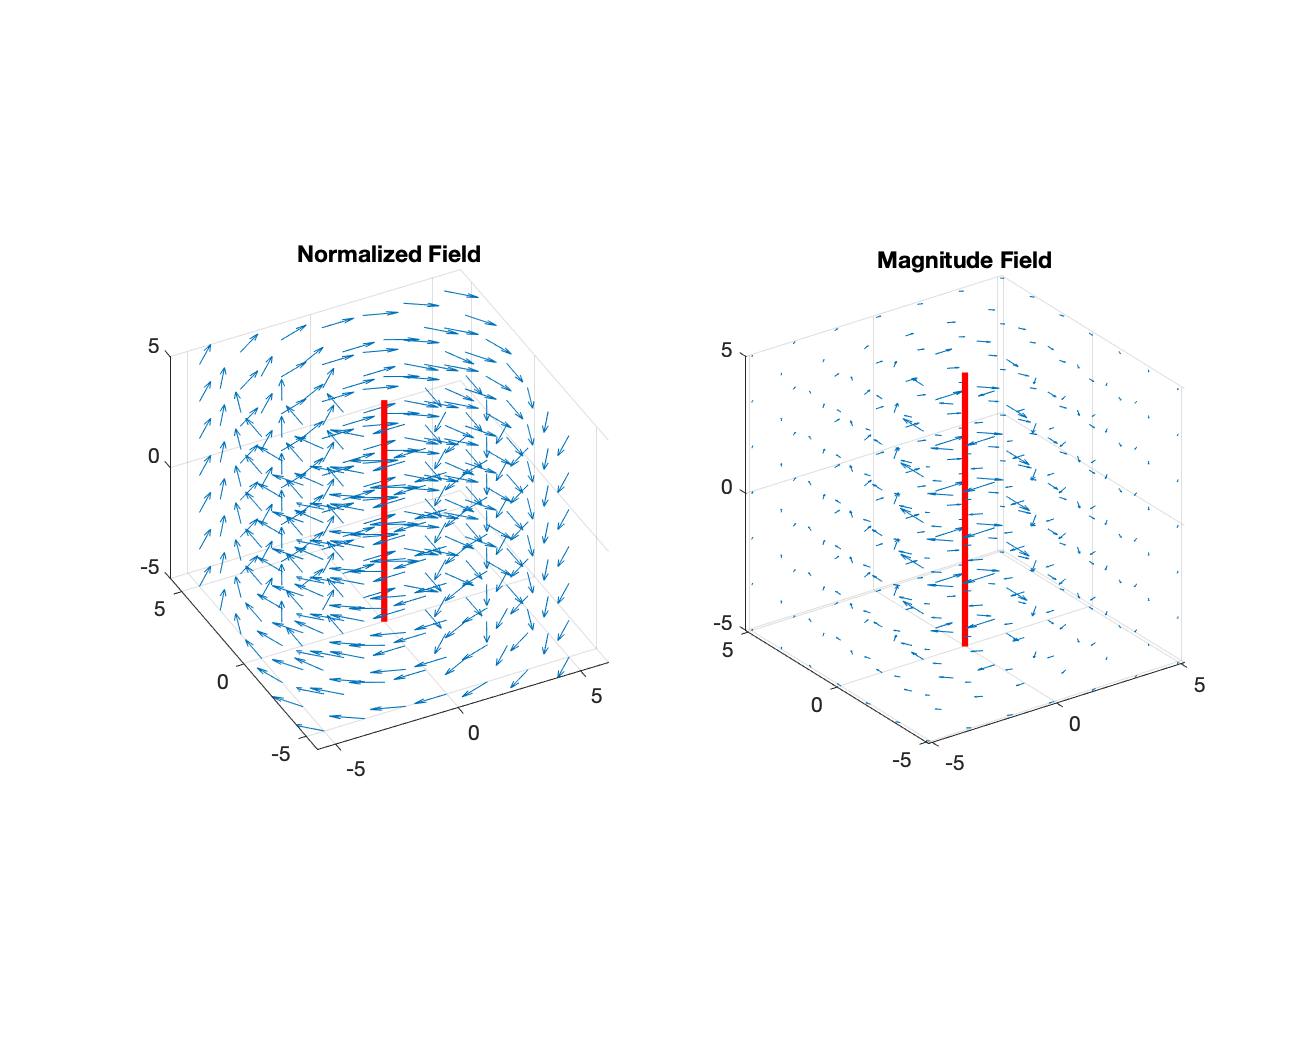
\includegraphics[width=\linewidth]{pics/linear.pdf}
    \caption{Магнитное поле протяженного провода}
\end{figure}

\begin{figure}[H]
    \centering
    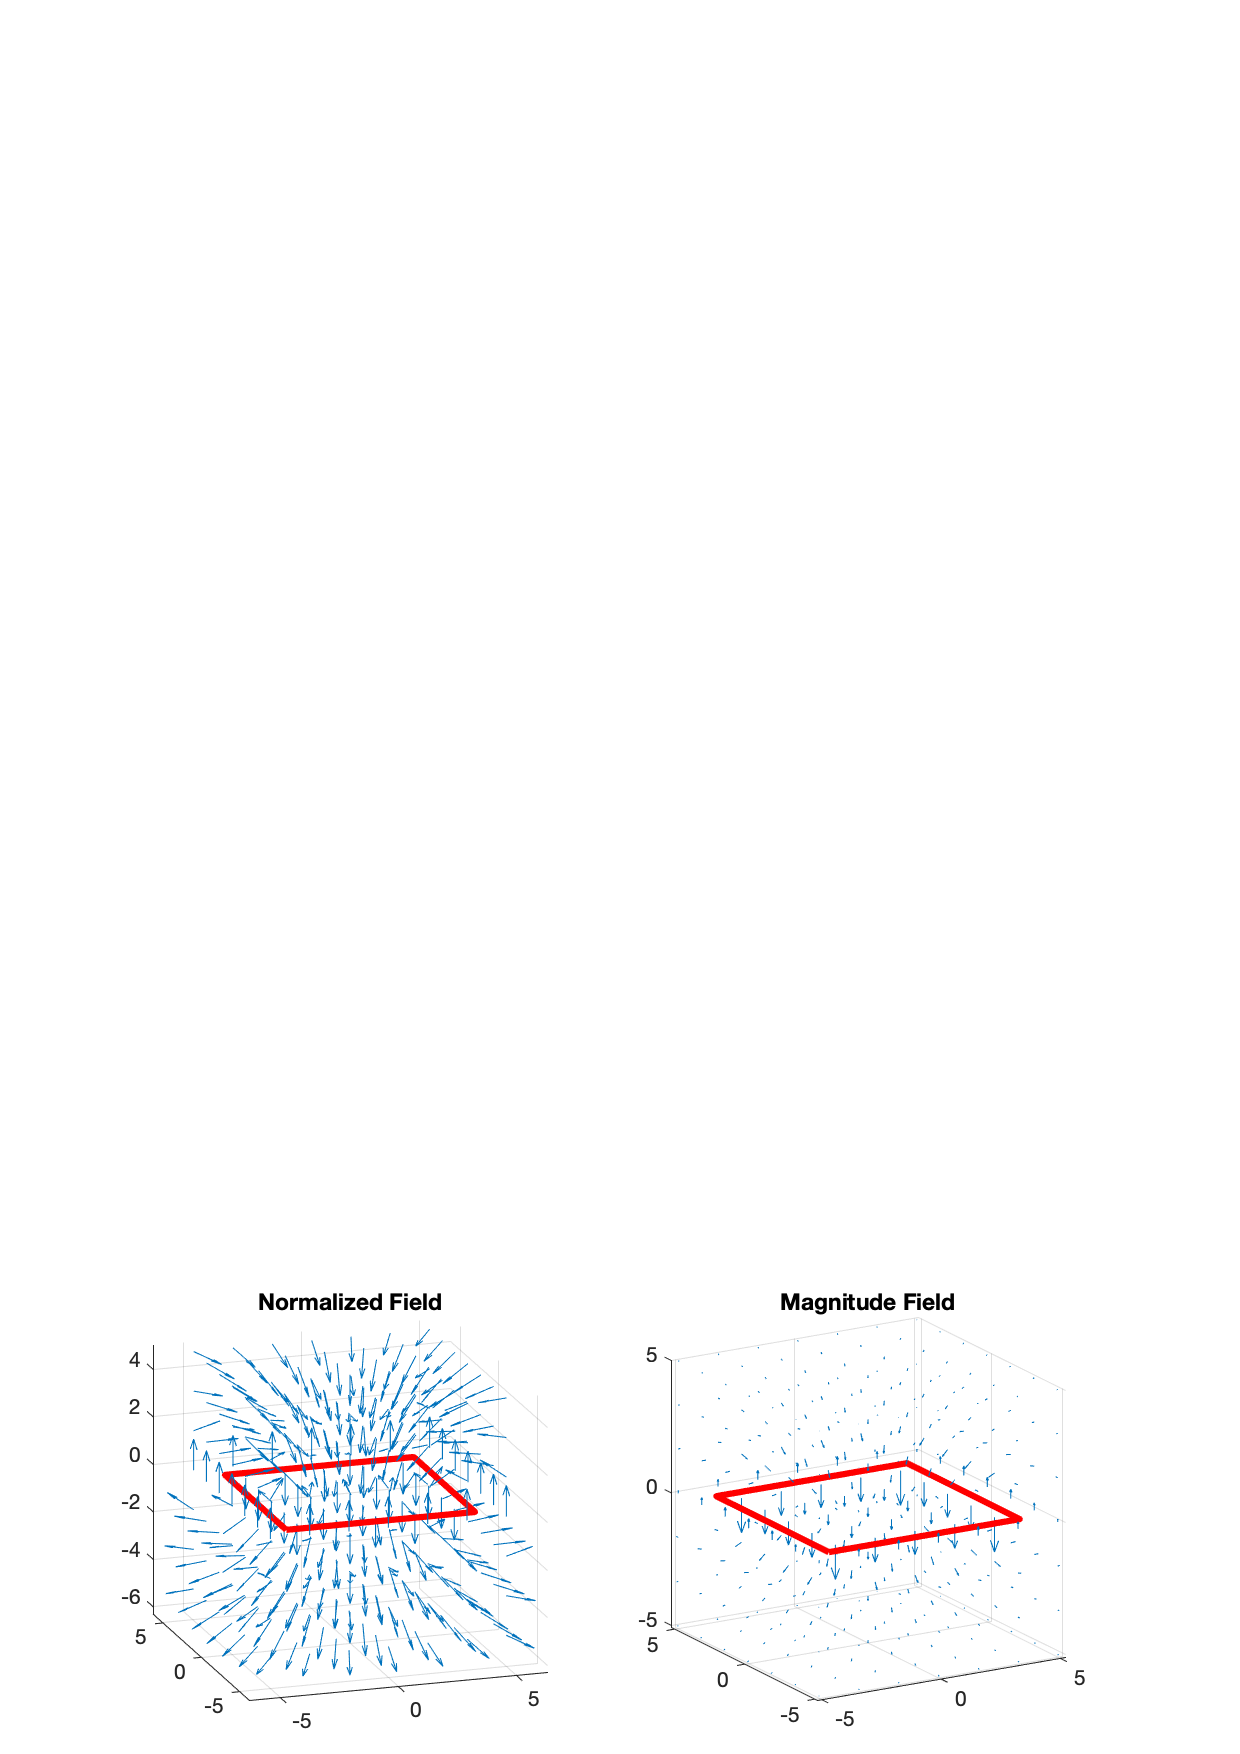
\includegraphics[width=\linewidth]{pics/square.pdf}
    \caption{Магнитное поле квадратной рамки}
\end{figure}

Промоделируем также поле соленоида (рис. 3)
\begin{figure}[H]
    \centering
    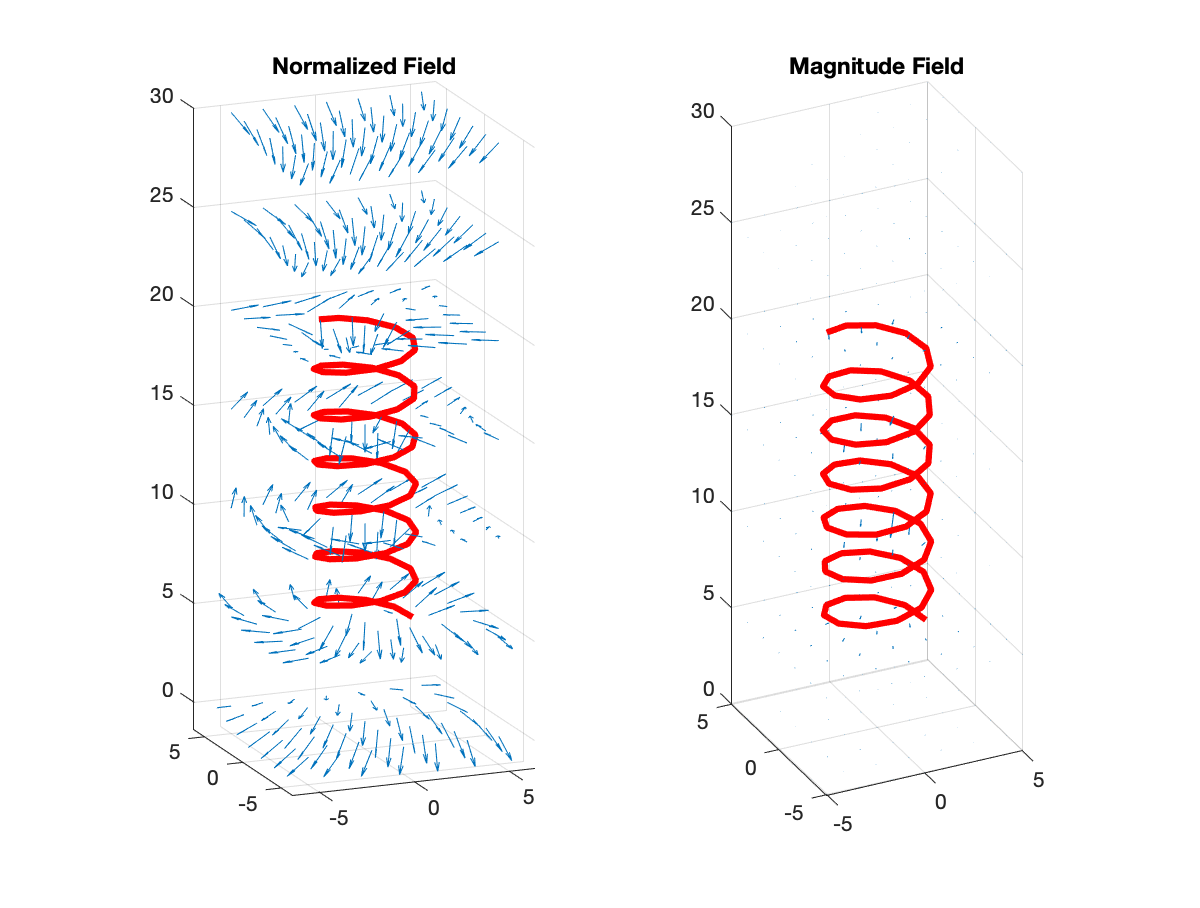
\includegraphics[width=\linewidth]{pics/solenoid.eps}
    \caption{Магнитное поле соленоида}
\end{figure}
Из получившейся модели явно видно, что поле, создаваемое таким соленоидом невелико, а также наблюдаются искажения, связанные с неплотностью намотки.
При этом, с увеличением плотности намотки, поле все более становится похожим на поле обычного магнита (рис. 4).
\begin{figure}[H]
    \centering
    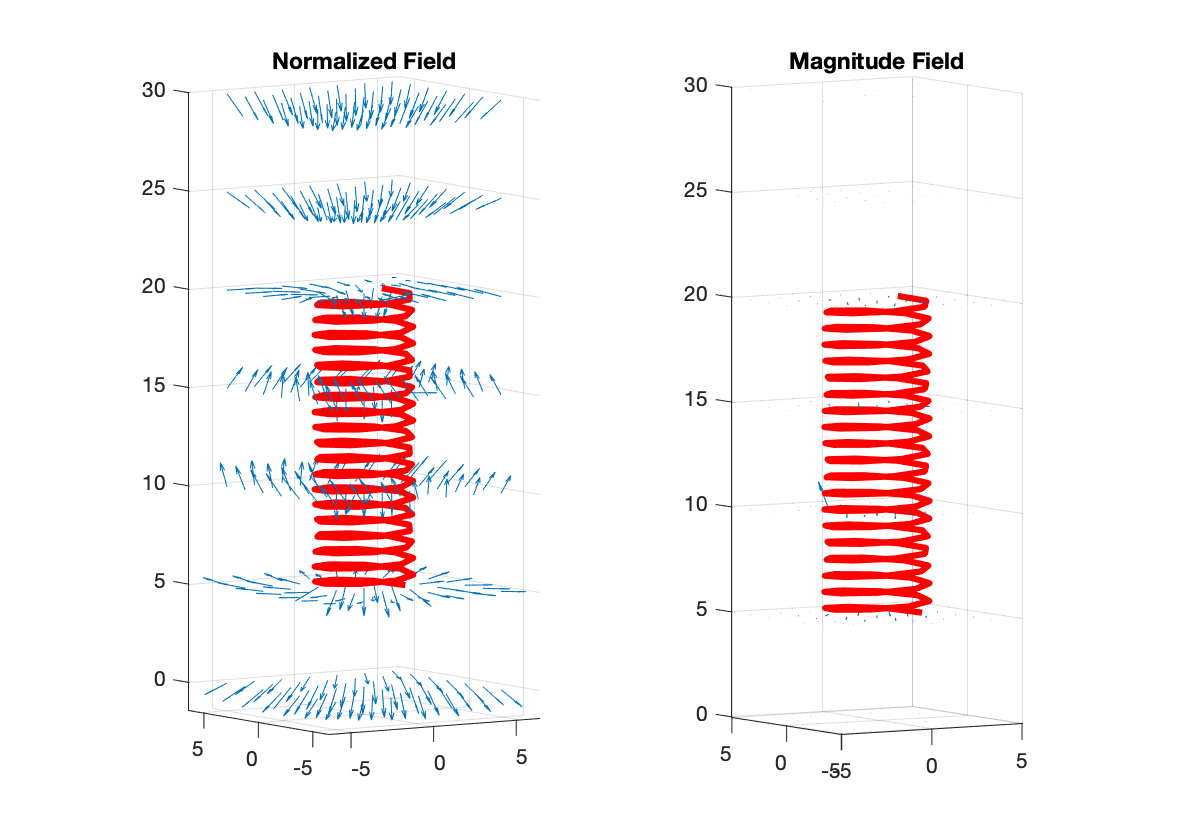
\includegraphics[width=\linewidth]{pics/solenoid2.eps}
    \caption{Магнитное поле соленоида}
\end{figure}

Также можно заметить, что поле, создаваемое соленоидом с переменным сферическим сечением, походит на поле вращающегося шара, подобно планетам (рис. 5).
\begin{figure}[H]
    \centering
    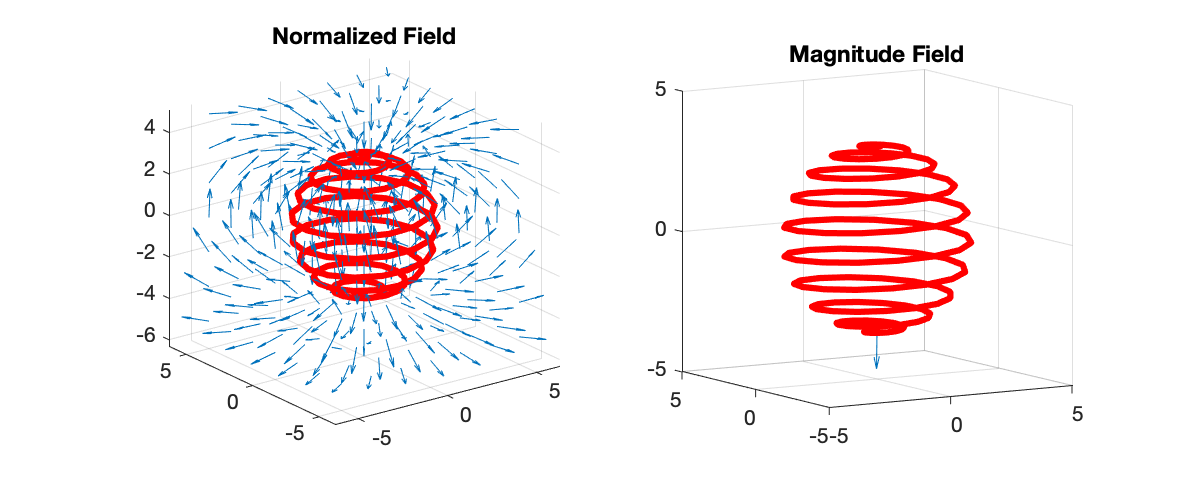
\includegraphics[width=\linewidth]{pics/sphere.eps}
    \caption{Магнитное поле сферичнского соленоида}
\end{figure}

Теперь, убедившись в корректной работе модели, можем пронаблюдать поле, создаваемое объектами различных несимметричных форм (рис. 6).
\begin{figure}[H]
    \centering
    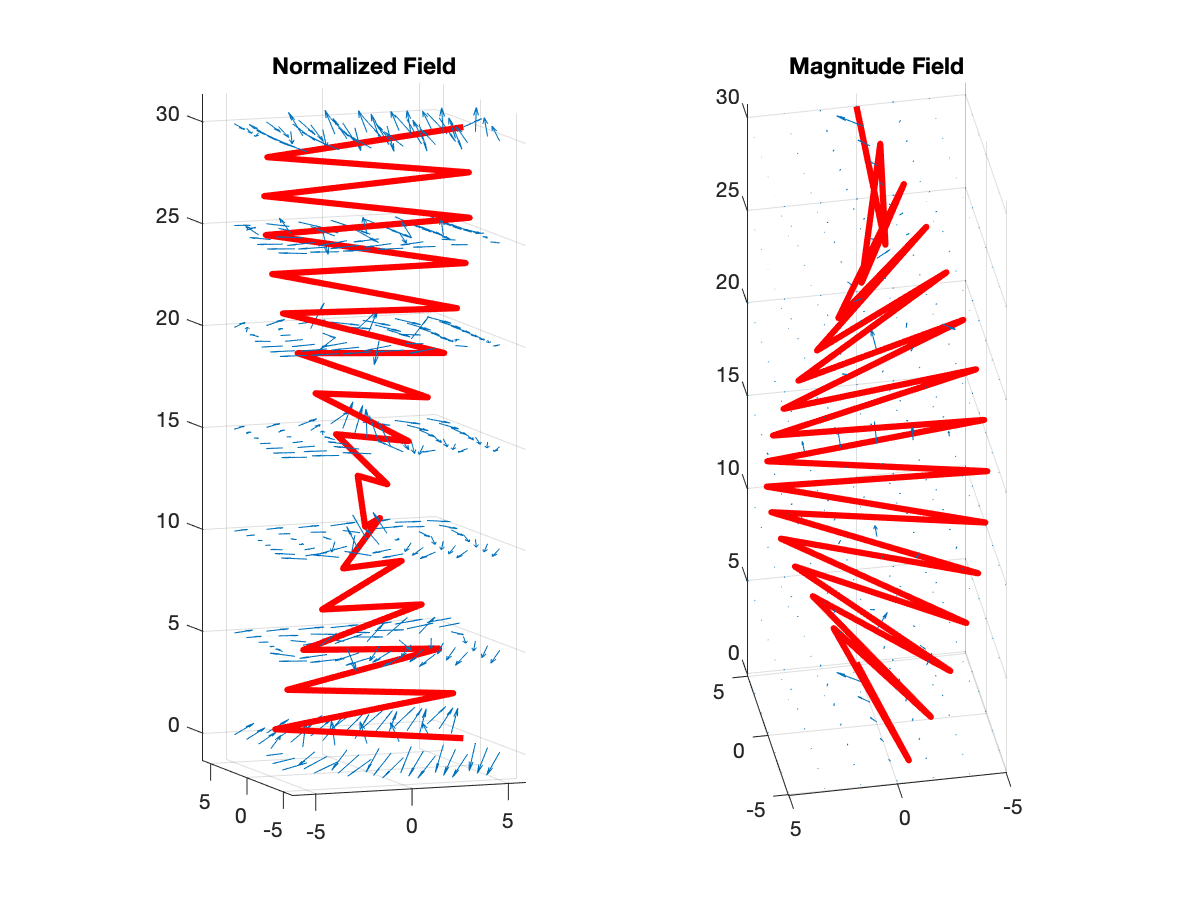
\includegraphics[width=\linewidth]{pics/gen.eps}
    \caption{Магнитное поле несимметричных объектов}
\end{figure}

\subparagraph*{Динамика заряженной частицы.}
Завершив моделирование поля, можем воспользоваться получившимися результатами для расчета траекторий заряженных частиц в поле различных объектов.
Взаимодействие частицы и поля можно описать формулой (7).

Далее, с помощью встроенного в среду MATLAB численного метода решения нежестких дифференциальных уравнений @ode45, можем получить выражение для искомой траектории (при этом все величины заранее обезразмерены). 
Будем отображать сразу несколько траекторий для частиц с разными начальными параматерами (скоростями).
По умолчанию программа предлагает возможность моделирования для протона, электрона и молекулы $O_2$, но пользователь может добавить новый тип частиц вручную.
После расчета и отображения наблюдаем следующие картины (траектории отображены только на левых изображениях, дабы не перегружать графики излишней информацией)

\begin{figure}[H]
    \centering
    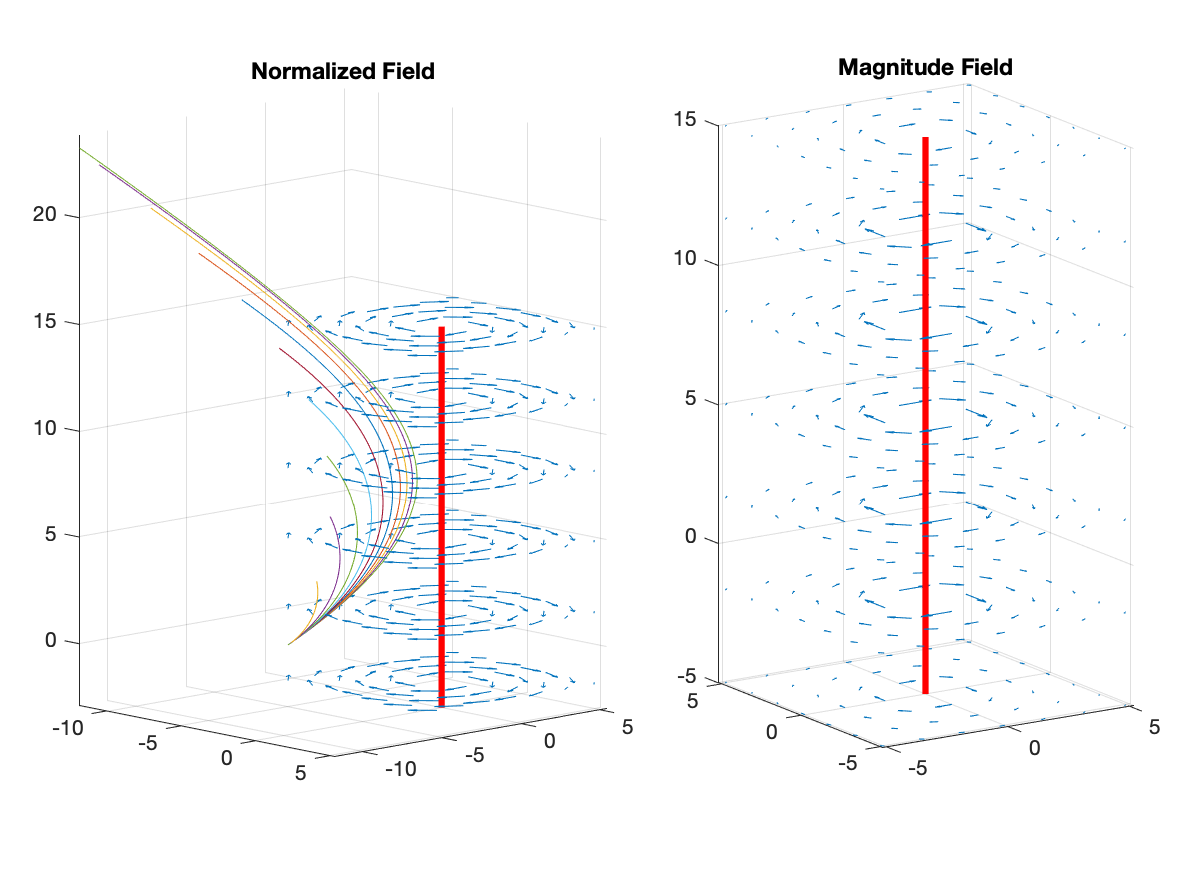
\includegraphics[width=0.8\linewidth]{pics/linear+q.eps}
    \caption{Протон в поле протяженного провода}
\end{figure}

Интересную картину можно увидеть в поле соленоида (рис. 8)
\begin{figure}[H]
    \centering
    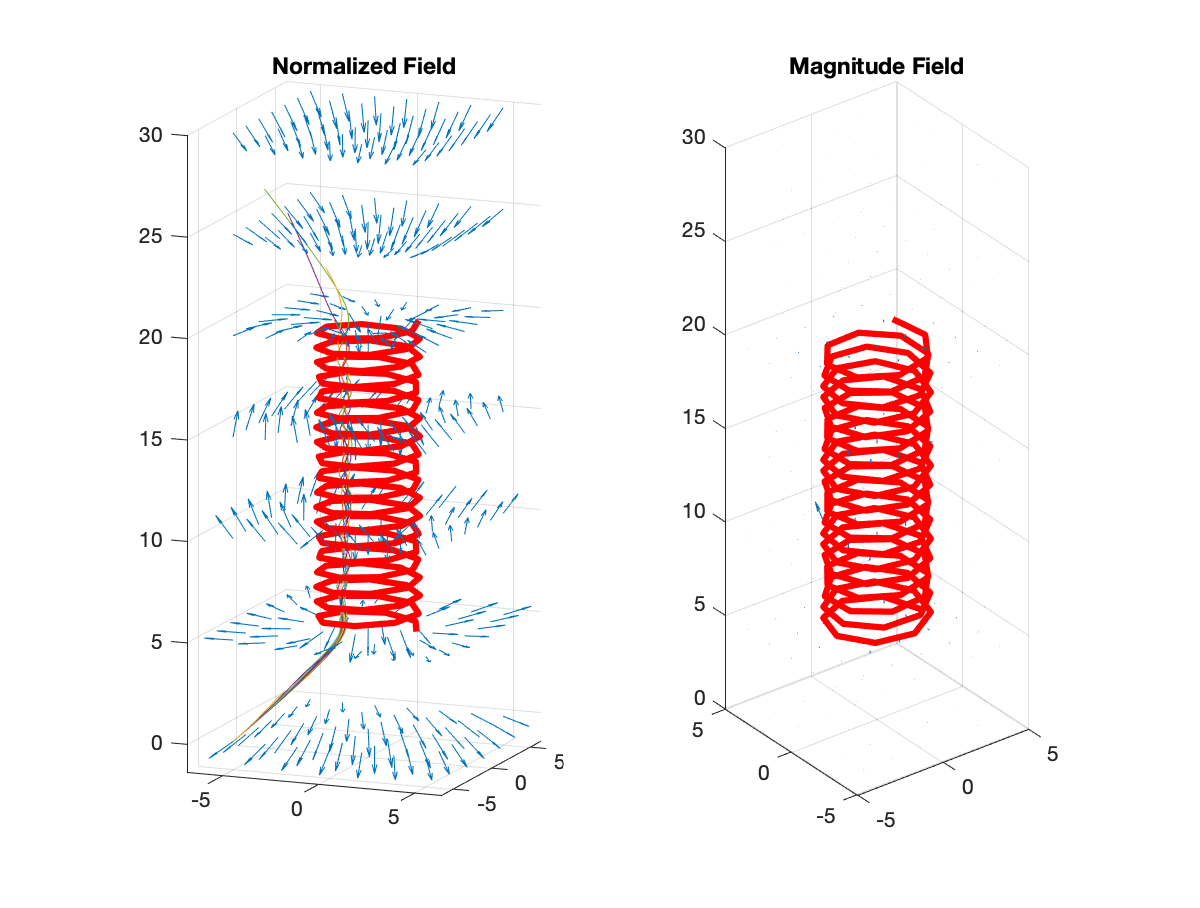
\includegraphics[width=0.85\linewidth]{pics/solenoid+q.eps}
    \caption{Протон в поле соленоида}
\end{figure}

Видно, что в центре катушки величина скорости почти не меняется (неточности есть в связи с недостаточной плотностью намотки), т.к. на оси поле сонаправлено скорости.

Также отобразим траекторию в поле сферы (рис. 9) и произвольного контура (рис. 10)

\begin{figure}[H]
    \centering
    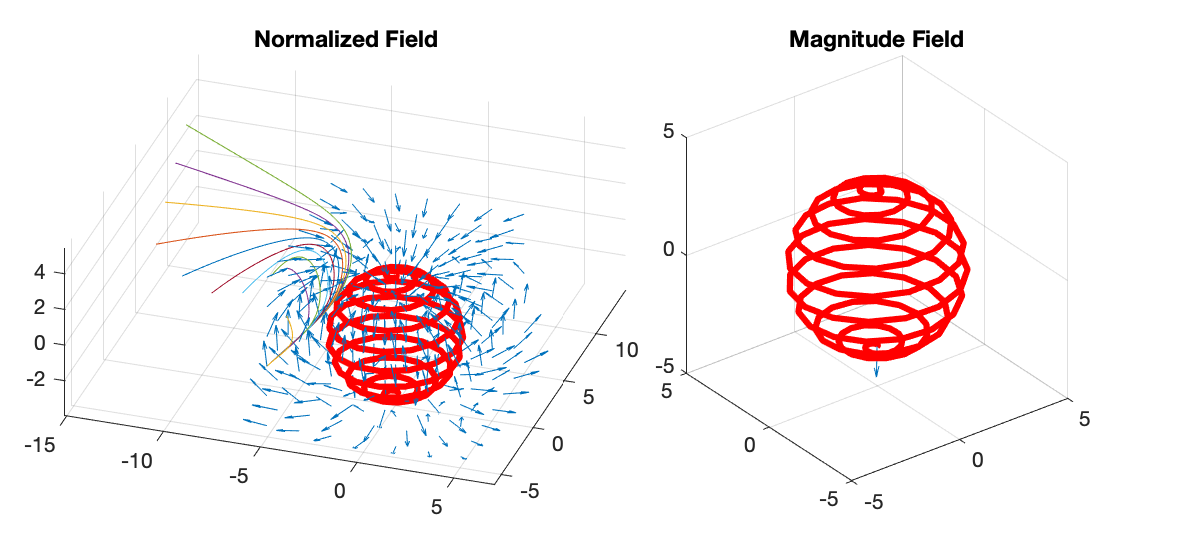
\includegraphics[width=\linewidth]{pics/sphere+q.eps}
    \caption{Протон в поле сферы}
    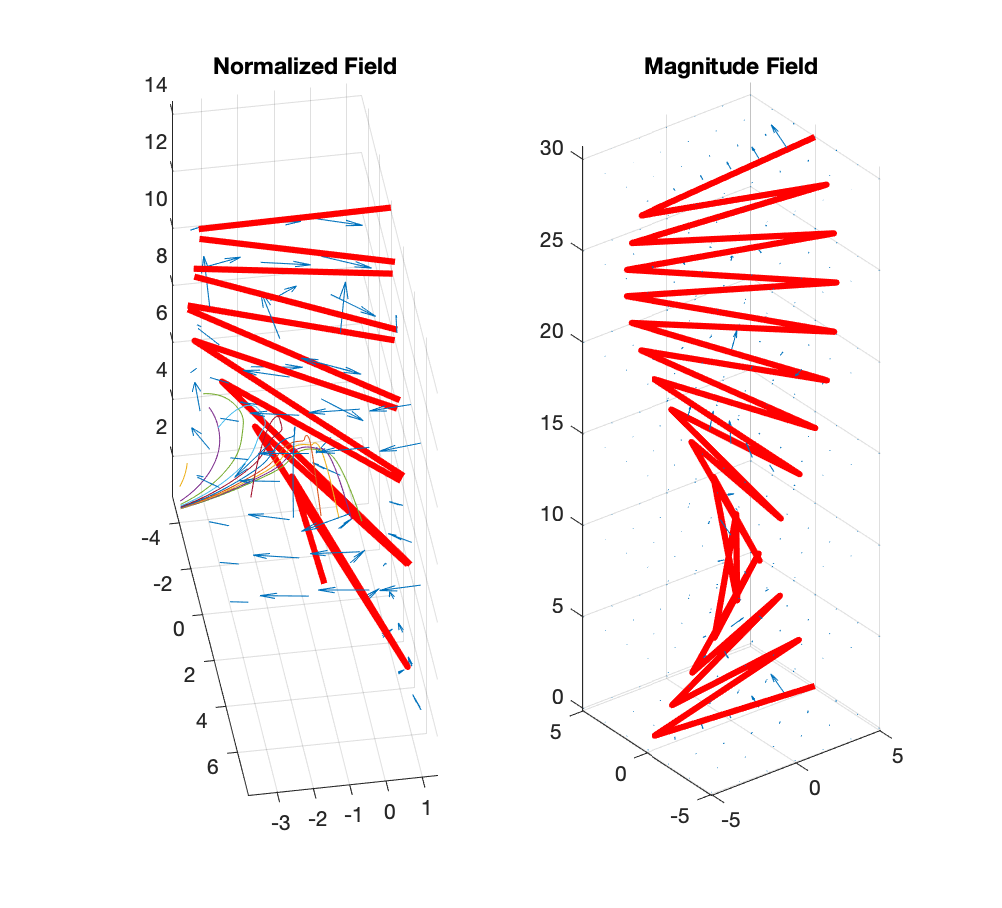
\includegraphics[width=0.9\linewidth]{pics/gen+q.eps}
    \caption{Протон в поле несимметричного объекта}
\end{figure}
\subsection*{Подведение итогов}
В ходе работы получена корректно работающая модель магнитного поля, создаваемого объектами различных форм.
Также промоделирована динамика заряженных частиц в полях рассматриваемых объектов.

Из преимуществ построенной модели можно отметить гибкость программы: присутствует возможность моделирования полей объектов самых различных форм, а при небольшой доработке и поля, создаваемые несколькими источниками.
Также из модели можно получать информацию как о направлении и форме поля, так и их величинах в каждой точке.
Также задавая различные начальные параметры частиц (координаты, скорости) можно наблюдать как меняется траектория и искать критические случаи.

Модель можно усовершенствовать возможностью добавления нескольких источников и, возможно, оптимизировав расчеты. 
Также присутствует небольшая неточность, проявляющаяся непосредственно на точках источника или в сильной близости к нему, где поле резко увеличивается, что вырождается в отдельные сильно выбивающиеся векторы, которые можно заметить на изображениях справа.
В будущем также можно рассмотреть движение релятивистских частиц и добавить в модель влияние полей, создаваемых самими частицами.
\end{document}
